\documentclass{article}

\usepackage[utf8]{inputenc}
\usepackage{geometry}
\usepackage{graphicx}
\usepackage{amsmath}
\usepackage{amsfonts}
\usepackage{hyperref}
\usepackage{setspace}
\usepackage{titlesec}

%tables
\usepackage{booktabs}
\usepackage{multirow}

%plot formatting
\usepackage{graphicx}
\usepackage{subcaption}

% Remove indentation
\setlength{\parindent}{0pt}

%margins for tables:
\newenvironment{custommargins}[2]{%
    \newgeometry{left=#1, right=#2}%
}{%
    \restoregeometry%
}

% Redefine the subsection format
\titleformat{\subsection}
  {\normalfont\itshape\large} % Format: italic and larger but not as large as section titles
  {\thesubsection} % Label
  {1em} % Separation between label and title
  {} % Before-code
\usepackage{booktabs}
\usepackage[table]{xcolor}
\usepackage{graphicx}
\doublespacing
% Document Setup
\title{Understanding the Gender Wage Gap: A Comparative Analysis of Income Disparities with Linear Regression}
\author{Jake Birnbach \and Khoa Dao \and Yan Mazheika}
\date{\today}

\begin{document}

\maketitle
\thispagestyle{empty}
\vspace{\baselineskip}
\vspace{\baselineskip}

\begin{abstract}
    Understanding the dynamics of individual income is crucial for developing effective economic policies and addressing inequality. Income disparities have been a central focus of socio-economic research, revealing mutual connections between factors such as gender, age, education, race, field of degree, and over time, the evolution of these relationships. This project seeks to explore the association between individual income and two pivotal factors: gender and geographic location.

A comprehensive analysis by the Human Resources for Health Journal on employees of the US Department of Health and Human Services from 2010 to 2018 demonstrates a narrowing yet persistent gender pay gap, emphasizing the role of location, job title, and supervisory responsibilities in this disparity. Despite adjustments for various factors, a residual gender pay gap remained, underscoring the complexity of addressing wage inequities \cite{HRfH}.  

Moreover, the geography of jobs significantly influences the gender wage gap, as revealed in a study published in the Federal Reserve Bank of Dallas. It was found that women's preferences for shorter commutes, coupled with the geographic concentration of high-wage jobs, exacerbate wage disparities. This relationship suggests that the spatial distribution of job opportunities plays a crucial role in continuing gender-based income differences. 

\end{abstract}

\section*{Introduction}
In recent decades, there’s been an ongoing debate concerning the equality of men and women regarding their pay. Within the 20th century, women’s participation in the labor force rose from roughly 10\% in the first decade of the 1900’s to 33\% in the decade following World War 2. Continuing this trend of growth, the current proportion of women in the civilian labor force has stabilized around 60\% \cite{BLSarticle}. Yet despite men and women participating in similar proportions in the labor force, many say that women are systematically discriminated against in the workforce.
\\

The wage gap is one of the most cited measures of this phenomenon and refers to the average disparity in income between men and women. While a portion of it can be explained through factors such as differences in age, education, skill level, etc., the rest of the gap is more difficult to explain and is often attributed to discrimination or other cultural reasons \cite{issuebrief}.
\\

In this project, we seek to understand, define, and quantify the different reasons men and women get paid differently. We’ll use sample data from surveys conducted in the 2000’s to represent the population of the United States. Our primary objective is to comprehend the wage gap and contextualize its significance. This entails analyzing income disparities between men and women across various age groups and geographic regions. Furthermore, in our examination of the factors contributing to the wage gap, we will attempt to quantify the extent of discrimination within the wage gap.
\\

Supporting this project, a study conducted on employees of the US Department of Health and Human Services between 2010 and 2018 sheds light on a narrowing yet persistent gender pay gap. This research underscores the impact of location, job title, and supervisory responsibilities on income disparities, suggesting that even after controlling for numerous variables, an unexplained gap persists \cite{HRfH}. Moreover, research from the Federal Reserve Bank of Dallas highlights the significant impact of job location on the gender pay gap. The study shows that women's preference for jobs closer to home, combined with the concentration of high-paying jobs in certain areas, heightens wage differences between genders. This suggests that the way job opportunities are geographically distributed plays a crucial role in the disparities observed in incomes \cite{DallasFed}. 

\vspace{\baselineskip}
\section*{Methods}
\subsection*{Description of Input Data}
We used the publicly available \href{https://usa.ipums.org/usa/}{IPUMS USA} dataset for sampling observations.
IPUMS provides census and survey data from around the world integrated across time and space. IPUMS integration and documentation makes it easy to study change, conduct comparative research, merge information across data types, and analyze individuals within family and community context. Data and services are available free of charge.
\\

More specifically, we used the recently compiled 2022 American Community Survey (ACS) for our analysis. The ACS consists of data for a wide variety of topics including peoples’ personal income, their education attainment, rent information, and more. Each observation represents a group of adults randomly sampled from the United States by mail who had the same response to the ACS survey questions. Weights are included to denote the frequency of a particular response. IPUMS USA allows for custom variable exportation of ACS datasets. The following features of interest were selected to export:
\vspace{\baselineskip}
\vspace{\baselineskip}

\begin{table}[!h]
    \centering
    \rowcolors{2}{gray!25}{white} % Alternate row colors starting from the second row
    \begin{tabular}{lp{6cm}}
        \toprule
        \textbf{Variable} & \textbf{Label} \\
        \midrule
        \textbf{PERWT} & Weights for Sample \\
        \textbf{SEX} & Sex \\
        \textbf{AGE} & Age \\
        \textbf{RACE} & Race \\
        \textbf{DEGFIELD} & Field of degree \\
        \textbf{EMPSTAT} & Employment status \\
        \textbf{UHRSWORK} & Usual hours worked per week \\
        \textbf{INCTOT} & Total personal income (\$) \\
        \textbf{PWSTATE2} & Place of work: state \\
        \bottomrule
    \end{tabular}
    \caption{Variables in Raw Dataset $N= 3,373,378$}
    \label{table:variables}
\end{table}

\subsection*{Data Cleaning}
Prior to regression modeling, the dataset was cleaned and re-coded. A description of the input data is provided in tables 2-3. Given the substantial size of the dataset, observations with missing values were dropped for the analysis. In addition, we decided to only include observations with employed individuals since our project aims at exploring a wage gap and unemployed individuals generally do not earn a wage. Several categorical variables were re-coded to ensure a more consise analysis. \textbf{DEGFIELD} was coded by aggregating similar degrees categories including STEM, Humanities, Business, Arts, etc (fill in other codes). Similarly, \textbf{PWSTATE2} was re-coded into regions including Central, Northeast, Northwest, Southeast, Southcentral,  and Southwest. This aggregation ensures less covariance when fitting the regression model, resulting in a more concise analysis. 
\\

Additionally, we transformed our dataset such that each observation now represents a single person. We achieved this by appending each row $n = \mathbf{PERWT}$ number of times to create a new weighted dataset which is used for the rest our analysis. The new dataset is significantly larger and contains $N = 61,636,706$ observations.

\begin{table}[ht]
    \centering
    \caption{Summary Statistics for Quantitative Variables}
    \begin{tabular}{@{}lccccccc@{}}
    \toprule
    Variable & Min & 1st Qu. & Median & Mean & 3rd Qu. & Max & Stdev \\ 
    \midrule
    INCTOT   & -8200 & 44400 & 73000 & 101179 & 119500 & 1640000 & 109138.29 \\
    AGE      & 19.00 & 32.00 & 42.00 & 43.32 & 53.00 & 95.00 & 13.27 \\
    UHRSWORK & 1.00 & 40.00 & 40.00 & 40.69 & 45.00 & 99.00 & 11.31 \\
    \bottomrule
    \end{tabular}
    \end{table}
    \newpage
    
    \begin{table}[ht]
    \centering
    \caption{Summary Statistics for Categorical Variables}
    \begin{tabular}{@{}lll@{}}
    \toprule
    Variable & Category & Proportion \\ 
    \midrule
    \multirow{2}{*}{SEX} & Female & 50.88\% \\
                         & Male & 49.12\% \\
    \midrule
    \multirow{9}{*}{RACE} & American Indian or Alaska Native & 0.42\% \\
                          & Black/African American & 8.62\% \\
                          & Chinese & 2.65\% \\
                          & Japanese & 0.37\% \\
                          & Other Asian or Pacific Islander & 7.56\% \\
                          & Other race, nec & 3.23\% \\
                          & Three or more major races & 0.70\% \\
                          & Two major races & 8.06\% \\
                          & White & 68.39\% \\
    \midrule
    \multirow{5}{*}{WORKREGION} & International & 0.05\% \\
                                & Midwest Region & 20.17\% \\
                                & Northeast Region & 22.73\% \\
                                & Other U.S. Territories and Special Areas & 0.77\% \\
                                & South Region & 32.36\% \\
                                & West Region & 23.92\% \\
    \midrule
    \multirow{13}{*}{DEGFIELD} & Arts and Design & 5.05\% \\
                               & Business and Industry & 22.55\% \\
                               & Communication and Media & 4.71\% \\
                               & Education and Teaching & 8.44\% \\
                               & Family and Consumer Studies & 0.72\% \\
                               & Health Sciences & 8.13\% \\
                               & Interdisciplinary Studies & 0.87\% \\
                               & Legal and Criminal Studies & 2.33\% \\
                               & Linguistics and Foreign Languages & 0.81\% \\
                               & Science and Environmental Studies & 2.14\% \\
                               & Social Sciences and Humanities & 21.42\% \\
                               & STEM & 22.82\% \\
                               & Technical and Vocational & 0.01\% \\
    \bottomrule
    \end{tabular}
\end{table}

\begin{custommargins}{2cm}{2cm}
\subsection*{Summary of Data}
\vfill
\begin{minipage}{0.49\textwidth}
    \centering
    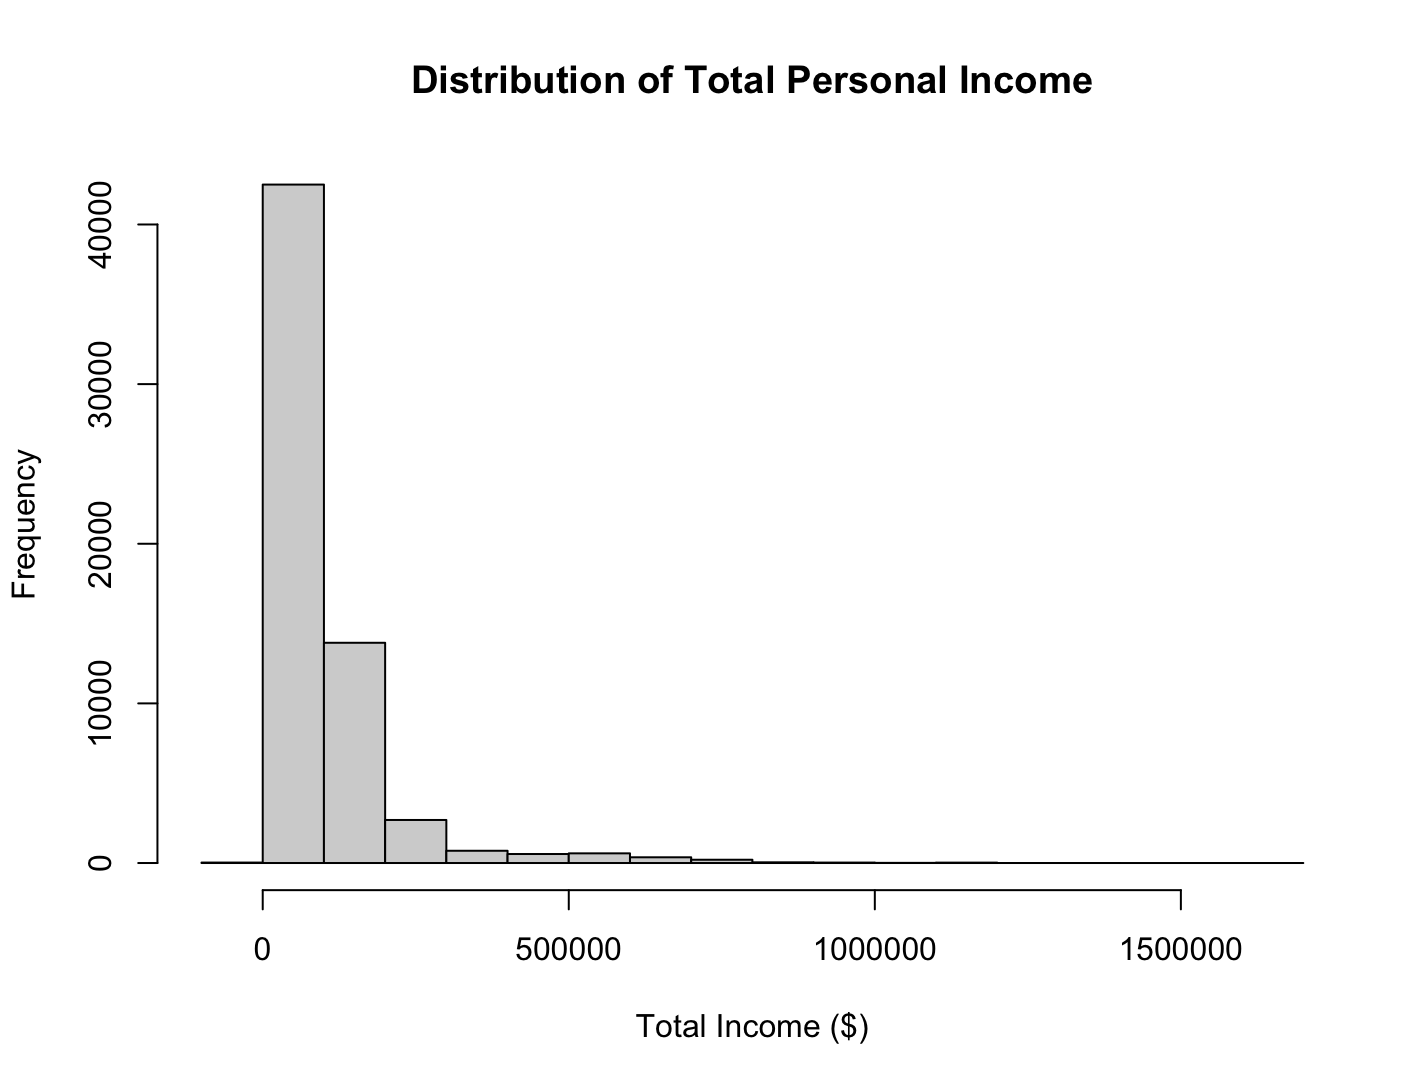
\includegraphics[width=\textwidth]{../figures/pre/Income_raw.png}
    \captionof*{figure}{\textit{Untransformed Income Distribution}}
\end{minipage}
\begin{minipage}{0.49\textwidth}
    \centering
    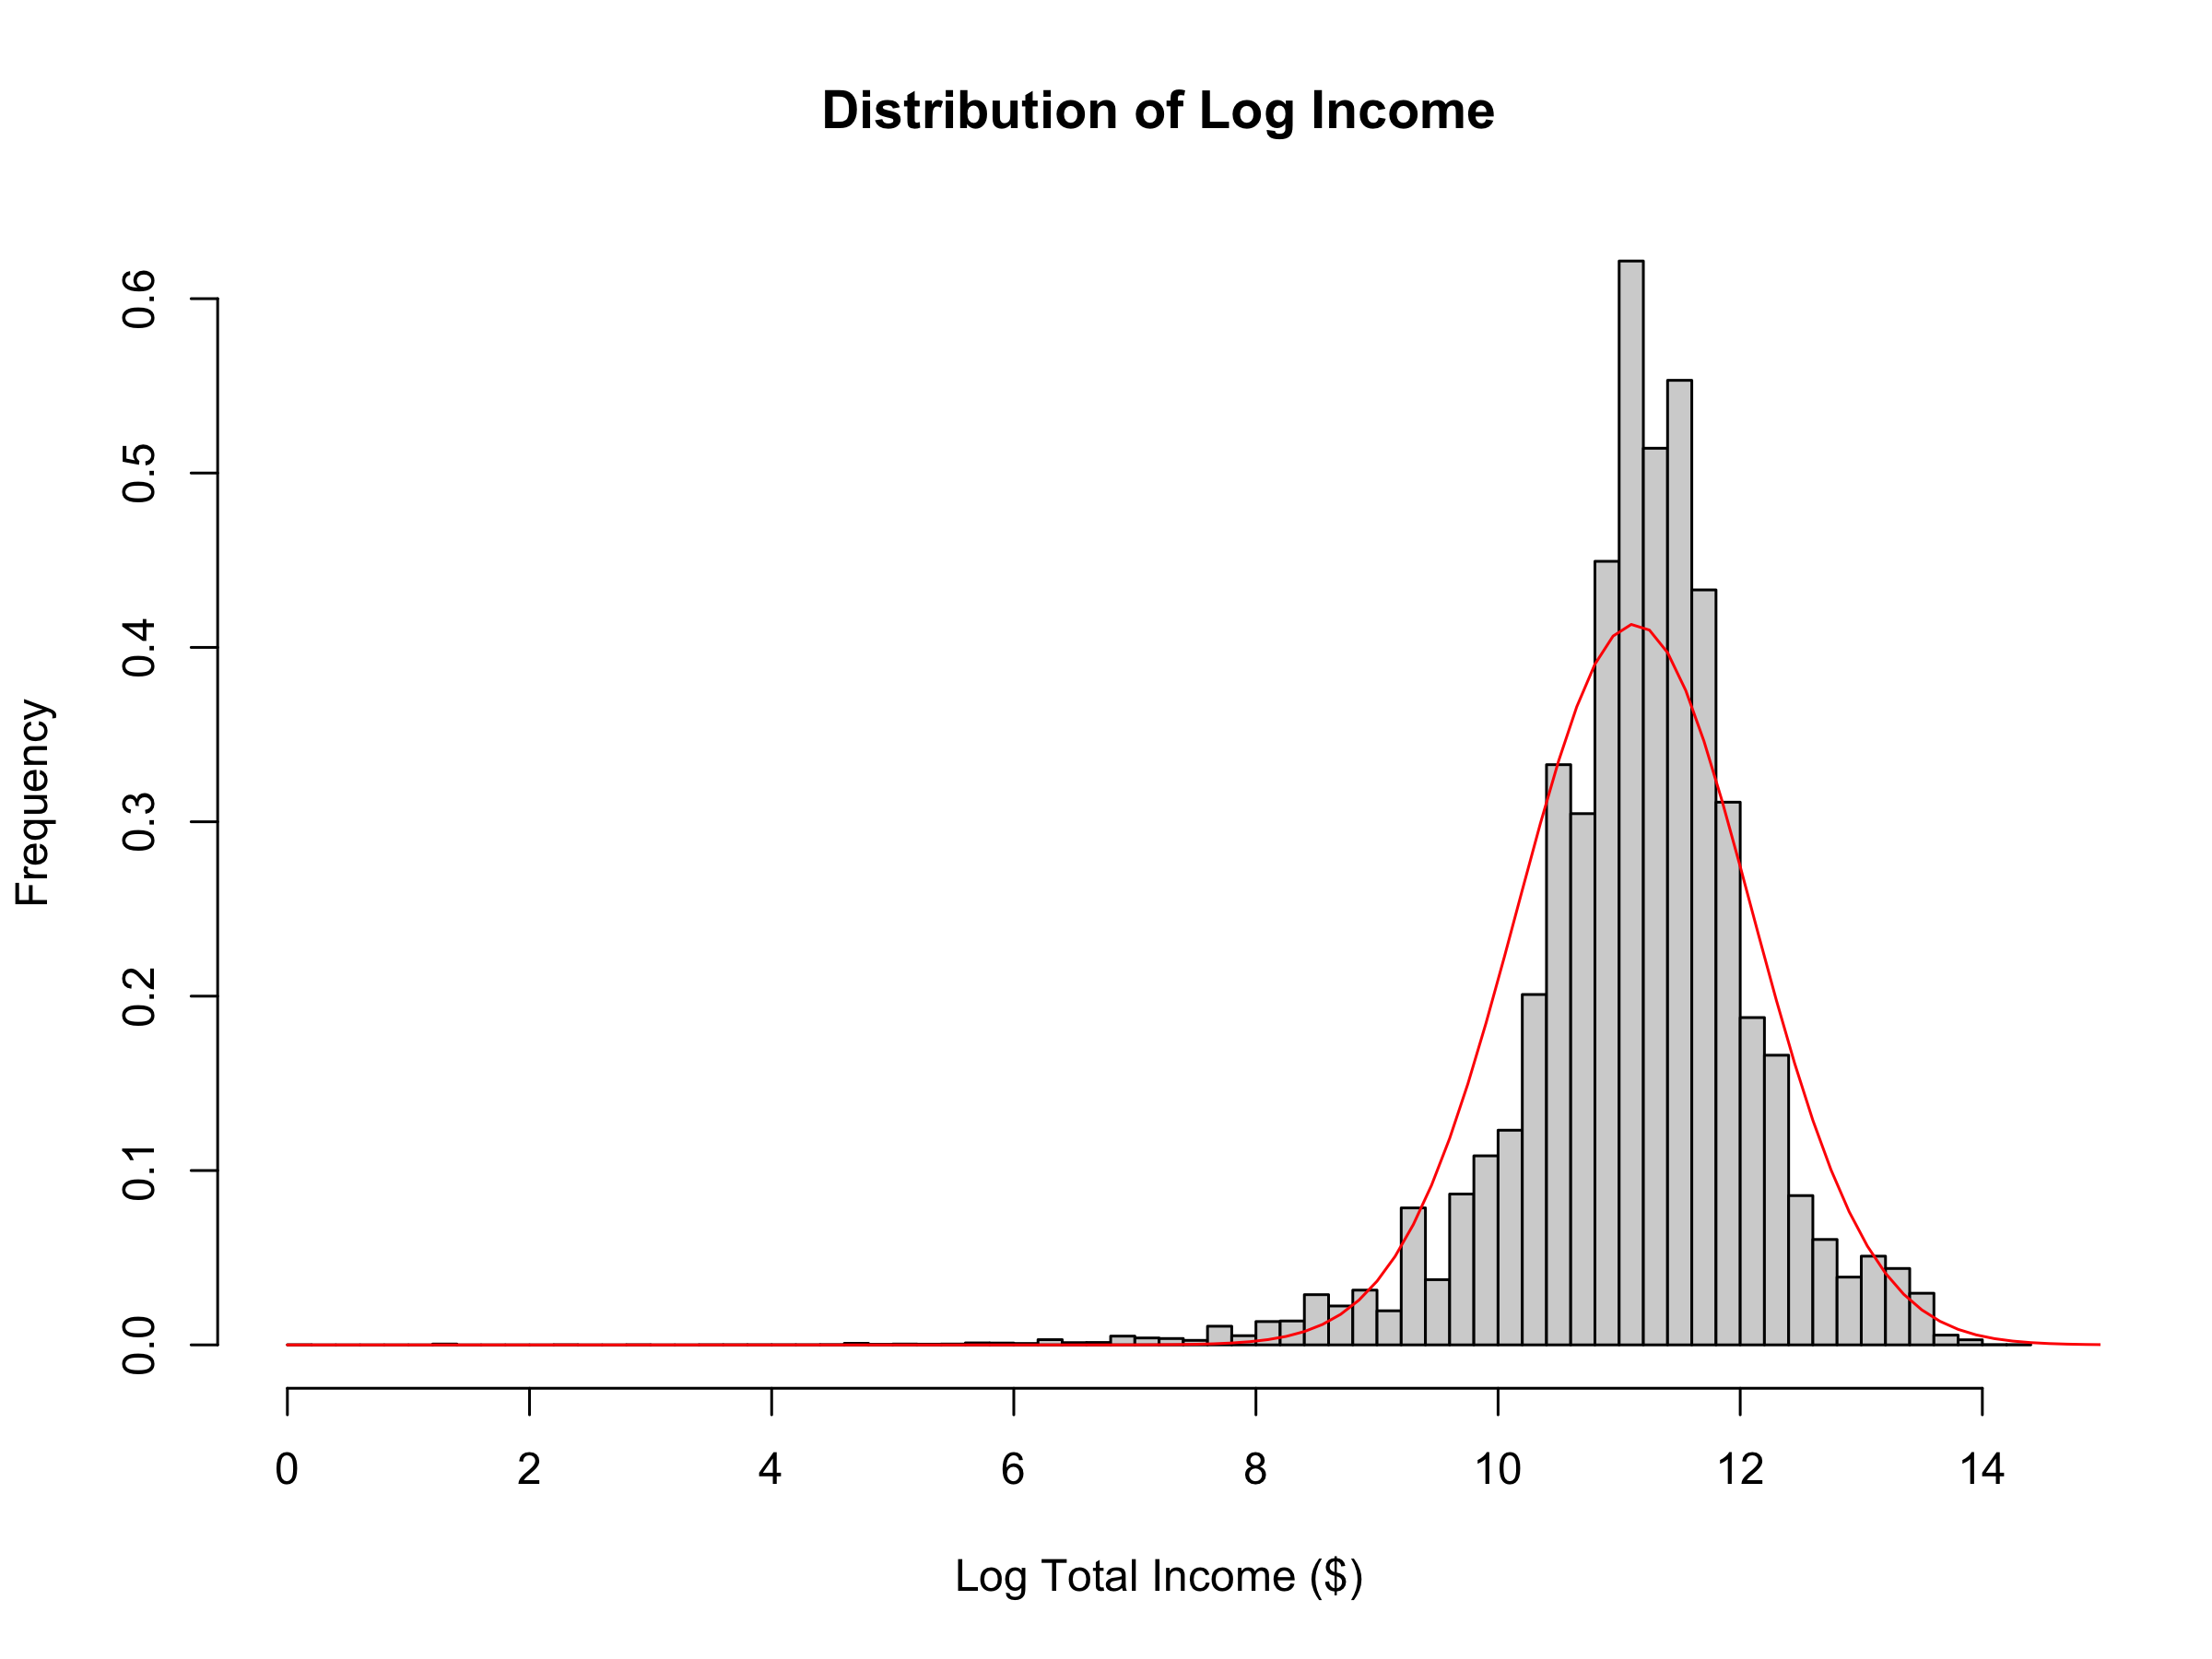
\includegraphics[width=\textwidth]{../figures/pre/loginc.png}
    \captionof*{figure}{\textit{Log-transformed Income Distribution}}
    \captionof*{figure}{\textit{with theoretical normal curve}}
\end{minipage}
\vfill
\begin{minipage}{0.49\textwidth}
    \centering
    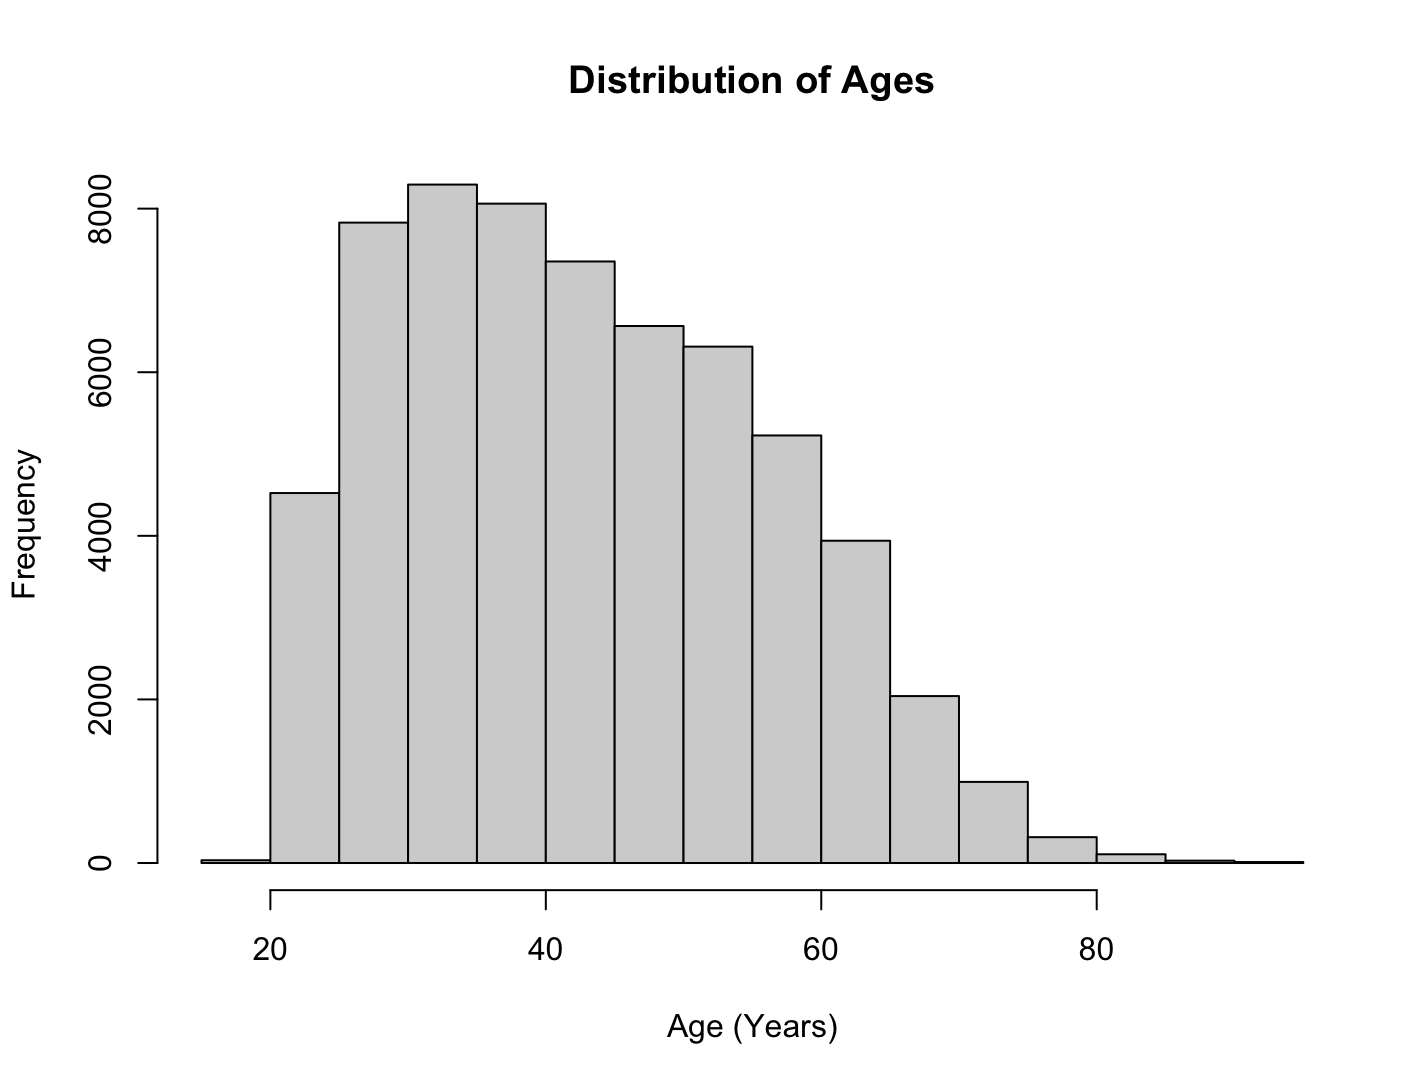
\includegraphics[width=\textwidth]{../figures/pre/age_plot.png}
    \captionof*{figure}{\textit{Age Distribution}}
\end{minipage}
\begin{minipage}{0.49\textwidth}
    \centering
    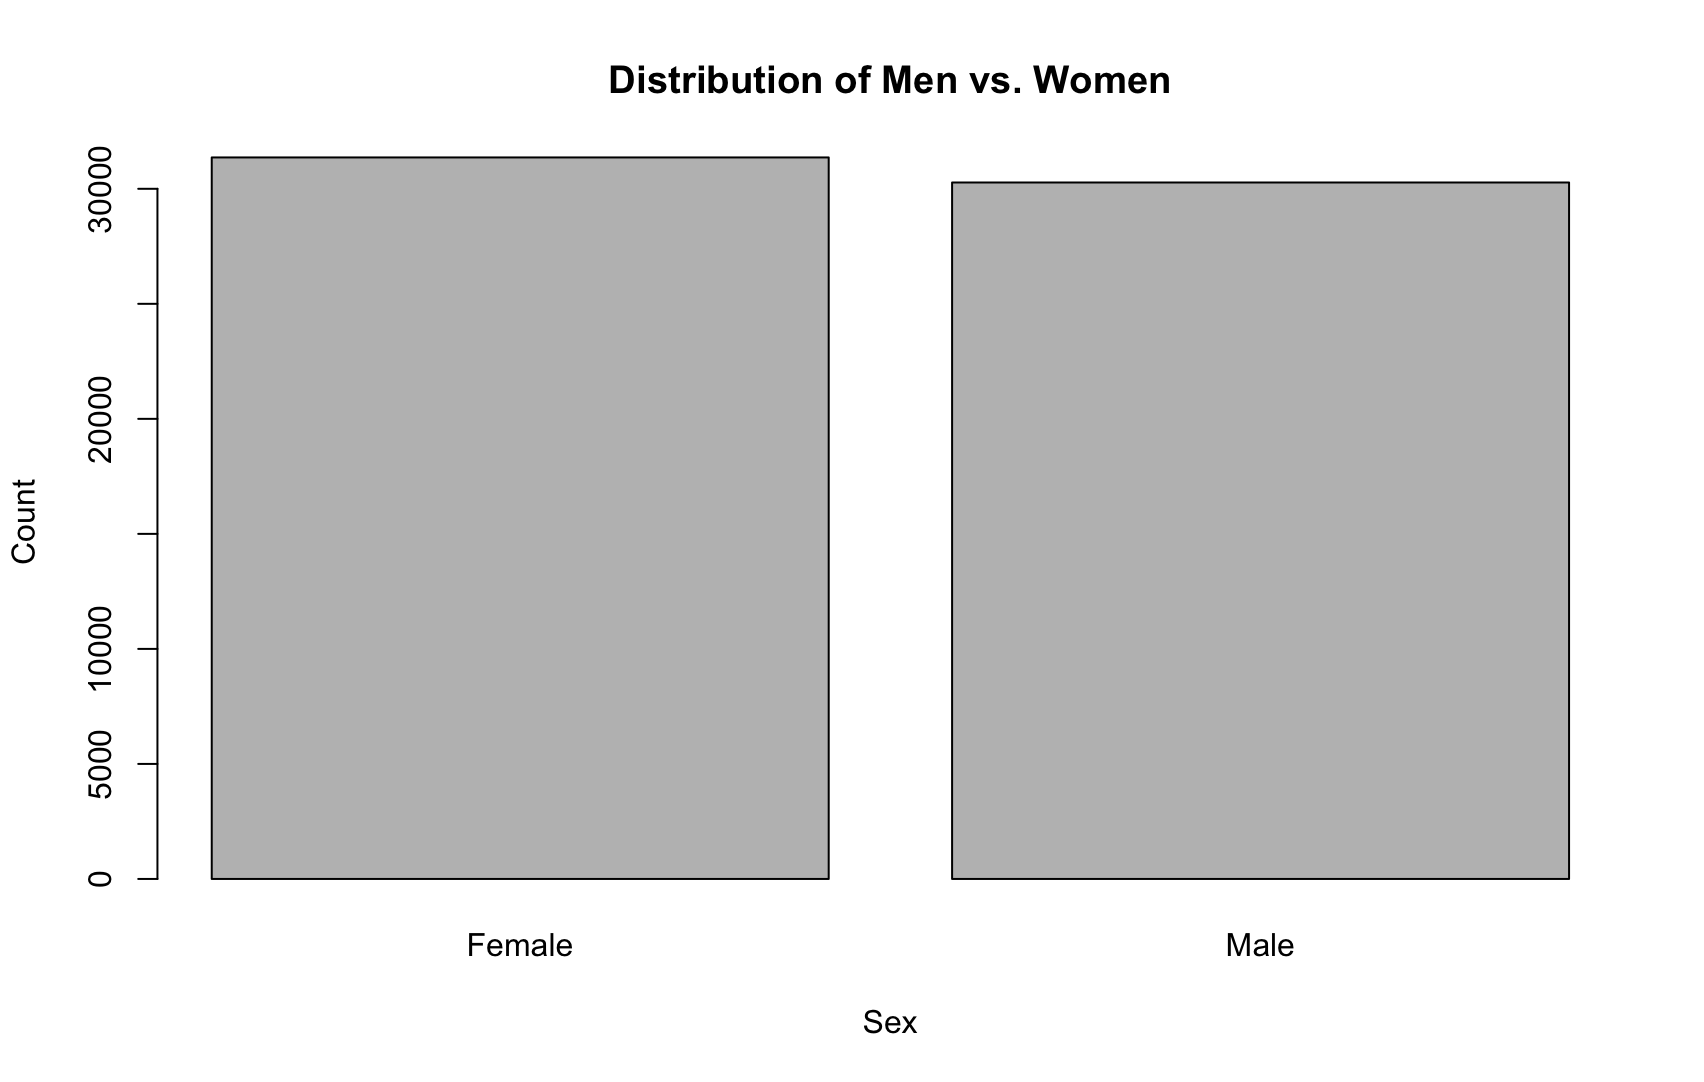
\includegraphics[width=\textwidth]{../figures/pre/sex_plot.png}
    \captionof*{figure}{\textit{Gender Distribution}}
\end{minipage}
\vfill
\begin{minipage}{0.49\textwidth}
    \centering
    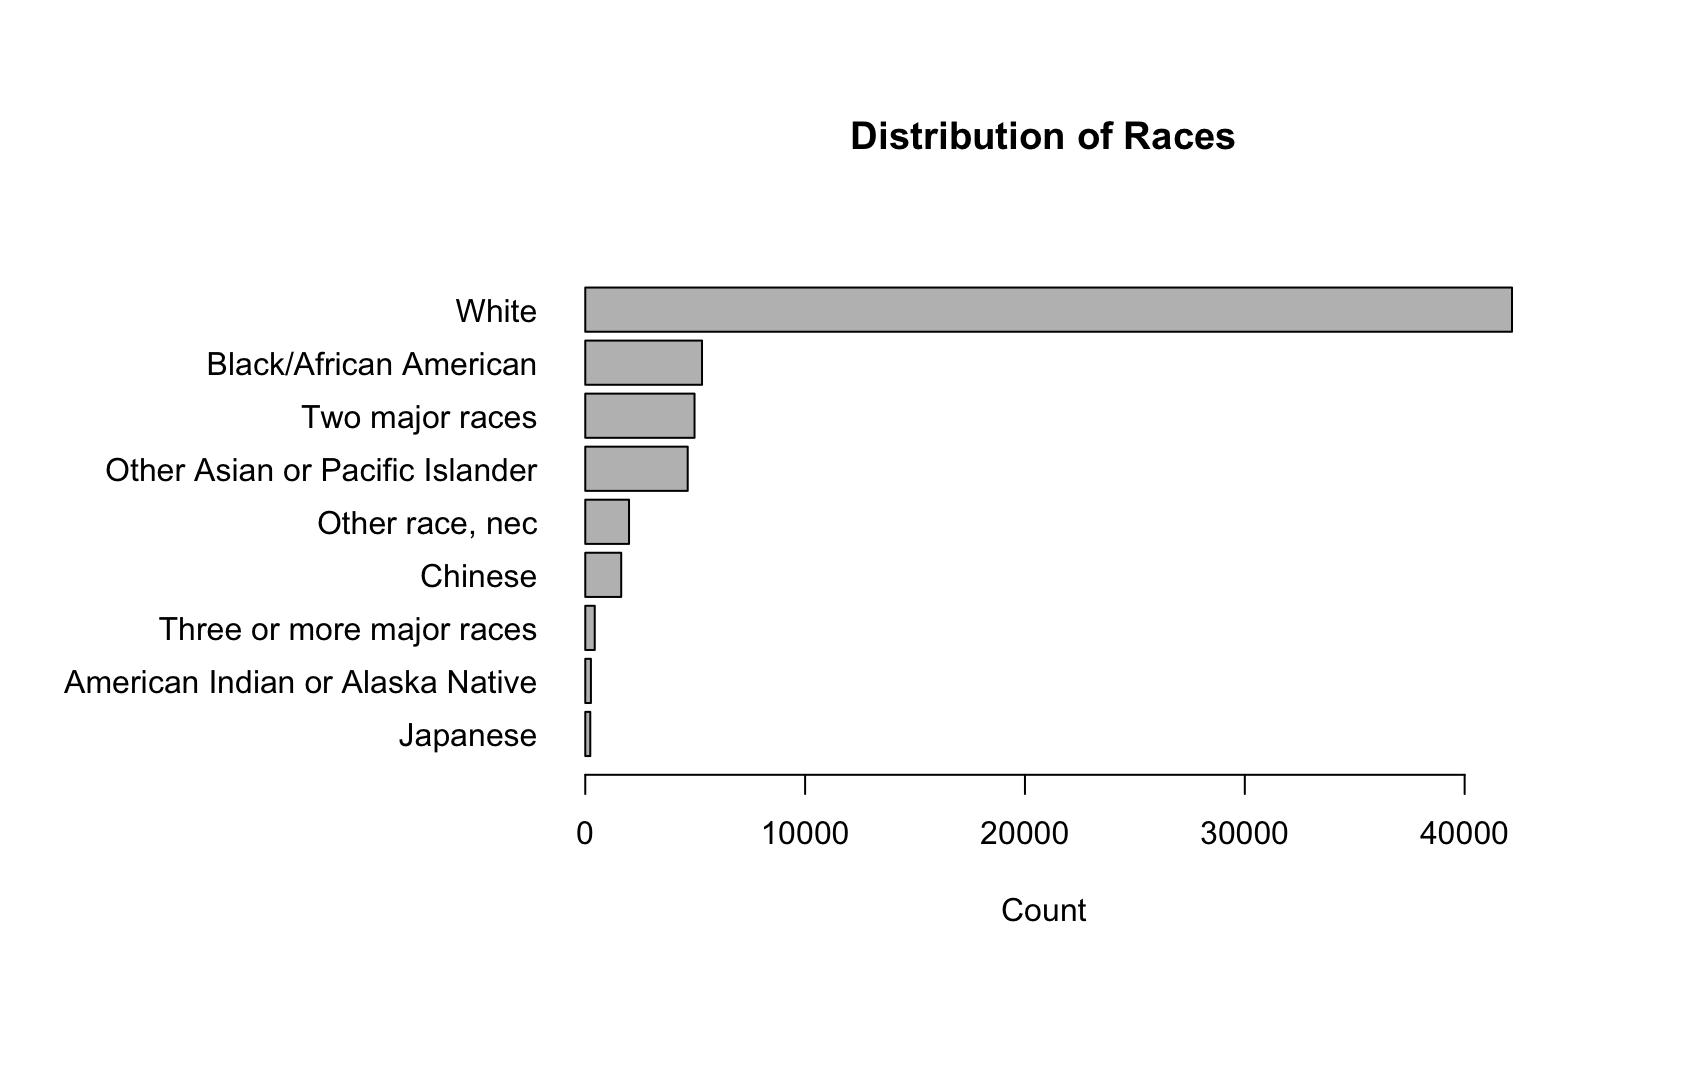
\includegraphics[width=\textwidth]{../figures/pre/race_plot.png}
    \captionof*{figure}{\textit{Race Distribution}}
\end{minipage}
\begin{minipage}{0.49\textwidth}
    \centering
    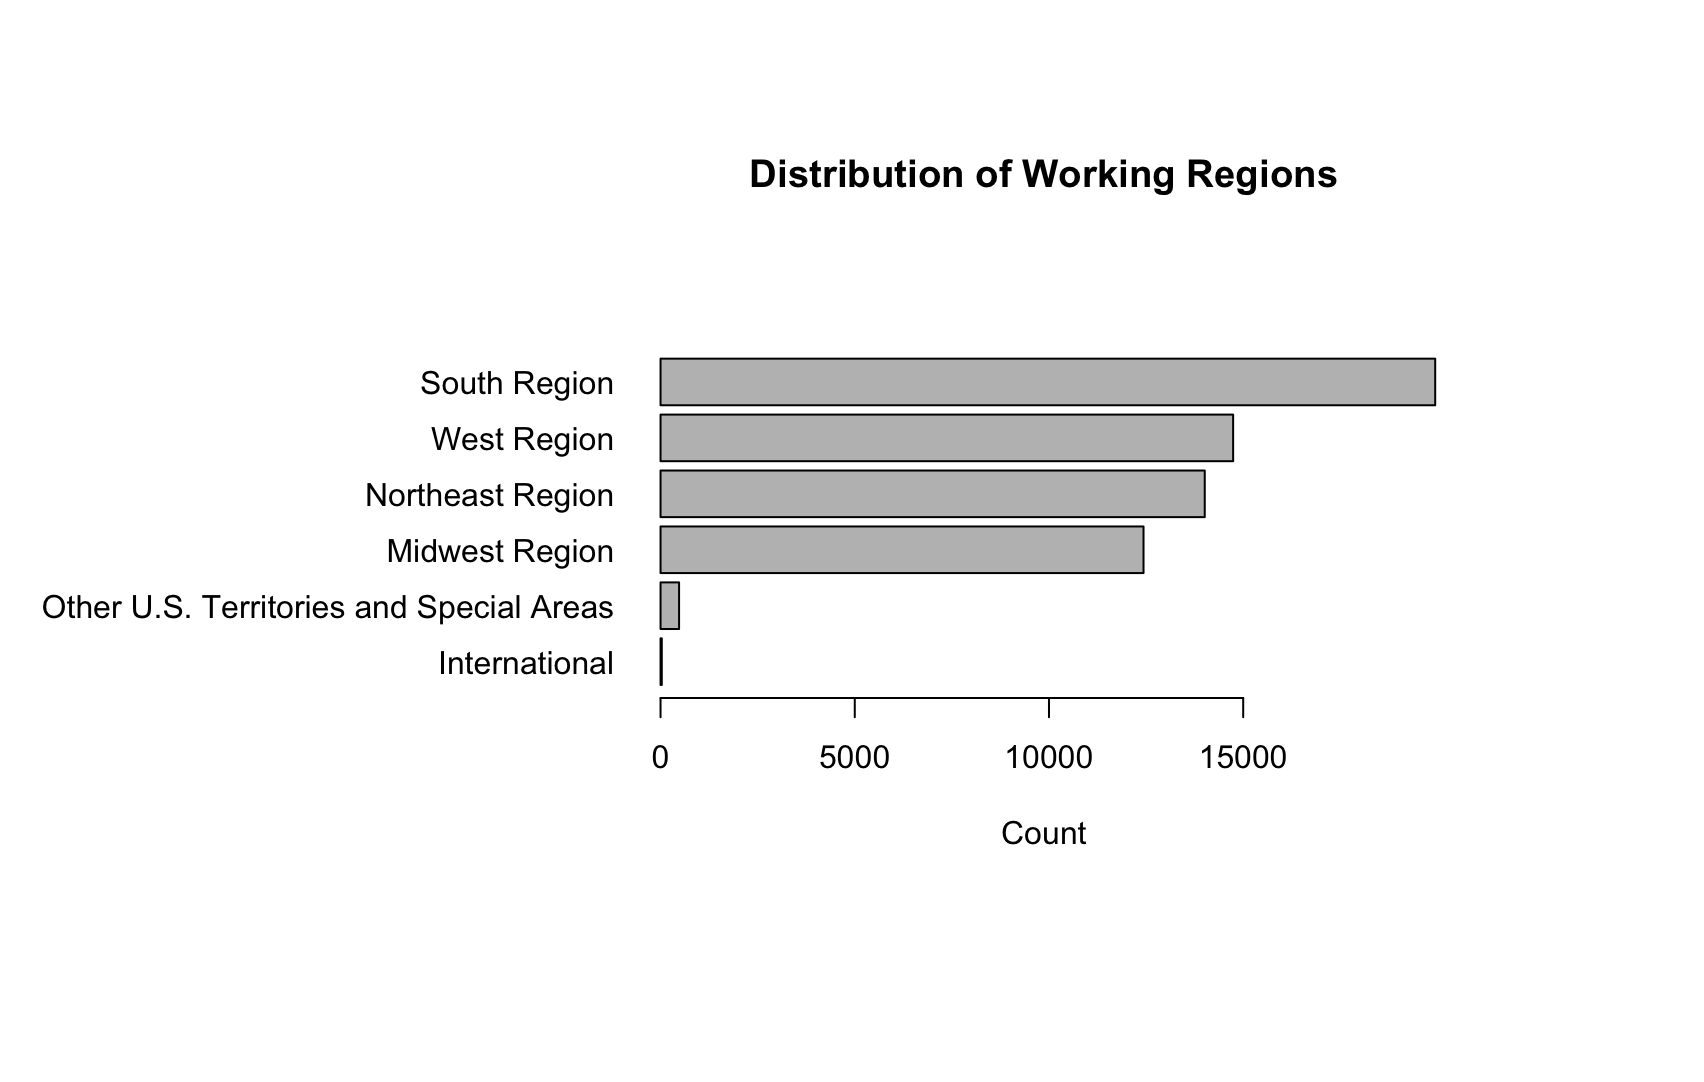
\includegraphics[width=\textwidth]{../figures/pre/work_region_plot.png}
    \captionof*{figure}{\textit{Work Region Distribution}}
\end{minipage}
\vfill
\begin{minipage}{0.49\textwidth}
    \centering
    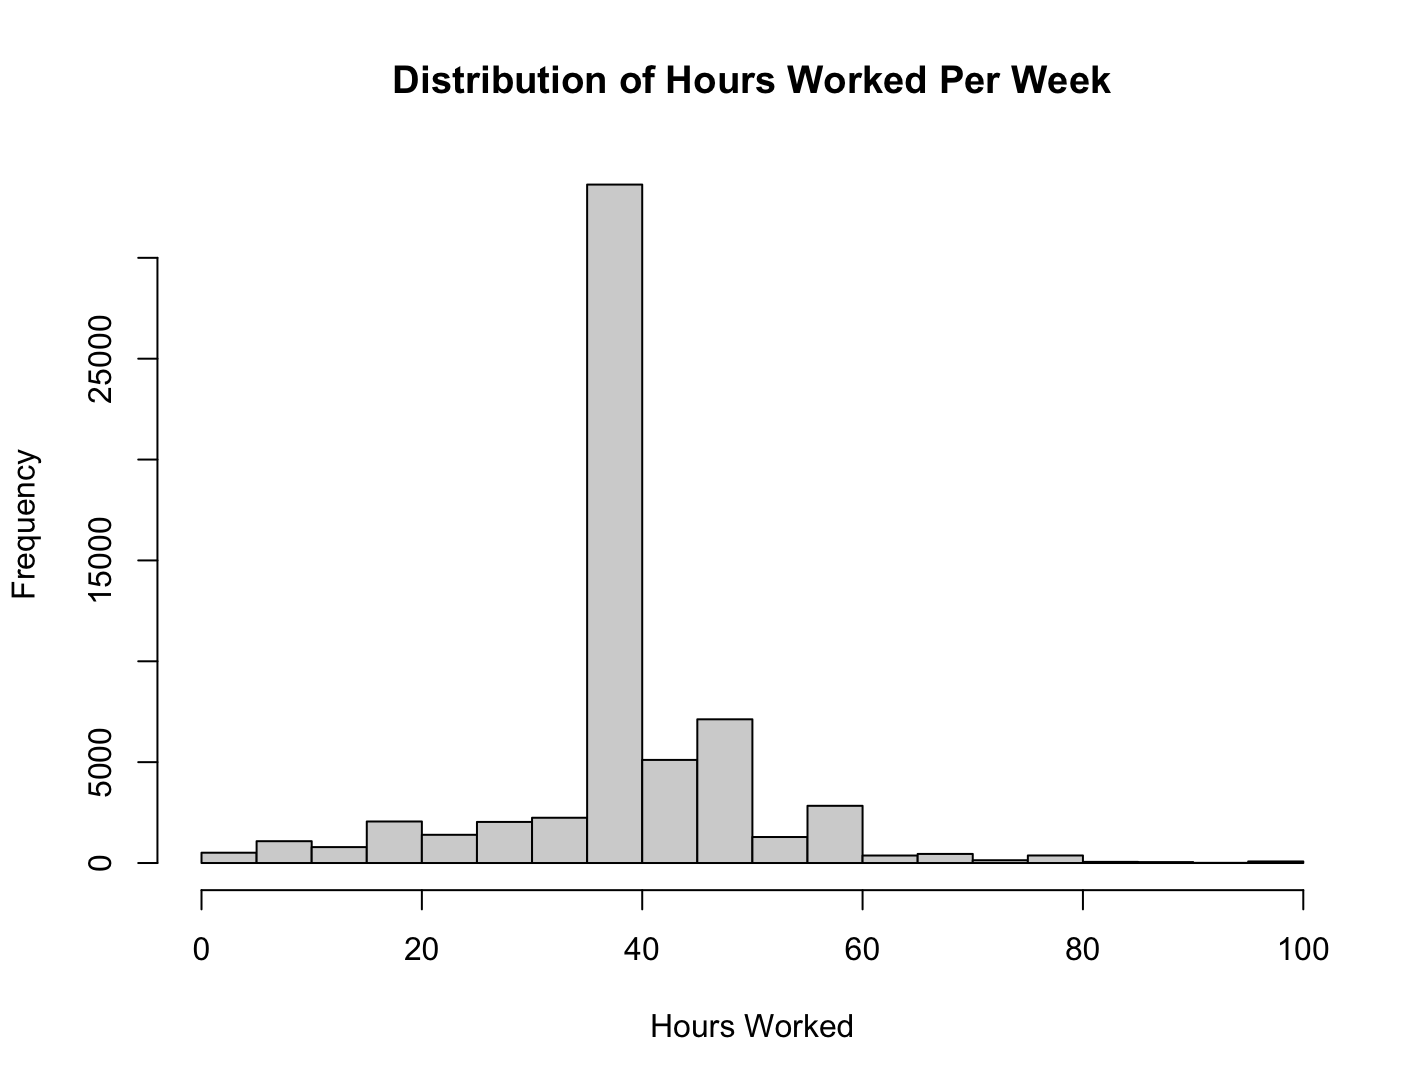
\includegraphics[width=\textwidth]{../figures/pre/hours_worked_plot.png}
    \captionof*{figure}{\textit{Hours Worked Distribution}}
\end{minipage}
\begin{minipage}{0.49\textwidth}
    \centering
    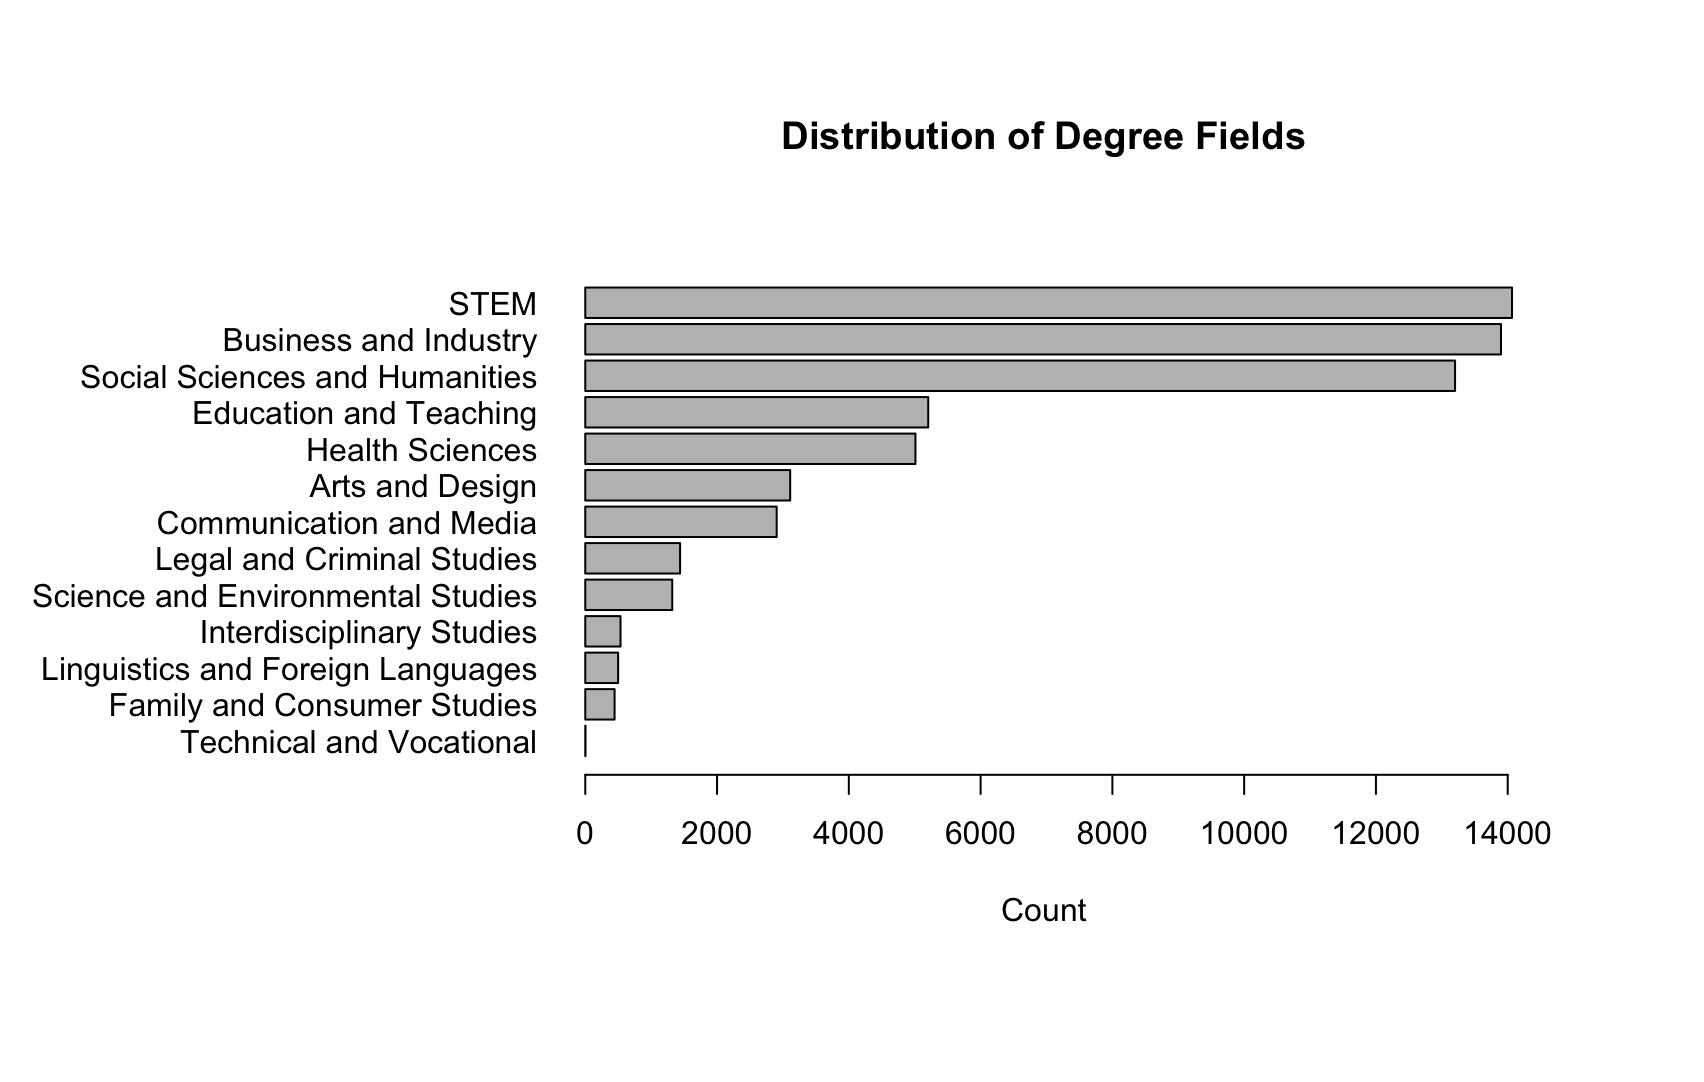
\includegraphics[width=\textwidth]{../figures/pre/deg_field_plot.png}
    \captionof*{figure}{\textit{Degree Field Distribution}}
\end{minipage}
\vfill

\end{custommargins}



\vspace{\baselineskip}
\subsection*{Creating the Model}
We created the following multivariate regression model to study how individual income is associated with sex and geographic location. 
% \begin{center}
% \texttt{INCTOT} = $\hat{\beta_0}$ + $\hat{\beta_1}$\texttt{SEX}
% \end{center}

% \noindent
% We'll then incorporate additional variables and ensure that they sufficiently correlate. For example,
\begin{center}
    \texttt{log(INCTOT)} = \texttt{AGE} + \texttt{AGE\textsuperscript{2}} + \texttt{SEX} + \texttt{RACE} + \texttt{WorkRegion} + \texttt{URSWORK}  + \texttt{DEGFIELD} + \texttt{AGE}*\texttt{SEX} + \texttt{AGE\textsuperscript{2}}*\texttt{SEX} + \texttt{SEX}*\texttt{RACE}
\end{center}
% And a more complex example:
% \begin{center}
%     \texttt{INCTOT} = \texttt{AGE} + \texttt{AGE\textsuperscript{2}} + \texttt{SEX} + \texttt{RACE} + \texttt{PWSTATE2} + \texttt{UHRSWORK} + \texttt{EDUC} + \texttt{DEGFIELD}
% \end{center}

% \noindent
Education features and hours worked will also be included in this regression to capture the difference in personal income for people in different fields, working different hours. We also included interaction terms between \texttt{AGE/AGE\textsuperscript{2}} and \texttt{SEX}, and  \texttt{SEX} and \texttt{RACE} to study whether different combinations of these features have a different effect on \texttt{INCTOT}.  These final models will be evaluated using Cross Validation and R-squared metrics. These empirical findings will inform whether there exists a significant income difference among people of different genders and race. 
\newpage
\section*{Findings}
\begin{table}[ht]
    \centering

    Summary of coefficients

    \begin{tabular}{rrrrr}
      \hline
     & Estimate & Std. Error & t value & Pr($>$$|$t$|$) \\ 
      \hline
    (Intercept) & 1.2934 & 0.2363 & 5.47 & 0.0000 \\ 
      AGE & -0.0412 & 0.0016 & -26.11 & 0.0000 \\ 
      `I(log(AGE\verb|^|2))` & 1.2611 & 0.0334 & 37.75 & 0.0000 \\ 
      SEXMale & 0.2392 & 0.0070 & 33.98 & 0.0000 \\ 
      `RACEBlack/African American` & 0.1233 & 0.0521 & 2.37 & 0.0180 \\ 
      RACEChinese & 0.3763 & 0.0547 & 6.87 & 0.0000 \\ 
      RACEJapanese & 0.2001 & 0.0742 & 2.70 & 0.0070 \\ 
      `RACEOther Asian or Pacific Islander` & 0.2879 & 0.0523 & 5.51 & 0.0000 \\ 
      `RACEOther race, nec` & 0.0247 & 0.0540 & 0.46 & 0.6477 \\ 
      `RACEThree or more major races` & 0.2188 & 0.0643 & 3.40 & 0.0007 \\ 
      `RACETwo major races` & 0.1811 & 0.0522 & 3.47 & 0.0005 \\ 
      RACEWhite & 0.3270 & 0.0510 & 6.41 & 0.0000 \\ 
      `DEGFIELDBusiness and Industry` & 0.2116 & 0.0163 & 13.02 & 0.0000 \\ 
      `DEGFIELDCommunication and Media` & 0.1158 & 0.0211 & 5.50 & 0.0000 \\ 
      `DEGFIELDEducation and Teaching` & -0.0389 & 0.0186 & -2.09 & 0.0364 \\ 
      `DEGFIELDFamily and Consumer Studies` & 0.0010 & 0.0414 & 0.02 & 0.9803 \\ 
      `DEGFIELDHealth Sciences` & 0.3127 & 0.0187 & 16.69 & 0.0000 \\ 
      `DEGFIELDInterdisciplinary Studies` & 0.2215 & 0.0382 & 5.80 & 0.0000 \\ 
      `DEGFIELDLegal and Criminal Studies` & 0.0892 & 0.0261 & 3.42 & 0.0006 \\ 
      `DEGFIELDLinguistics and Foreign Languages` & 0.1537 & 0.0393 & 3.91 & 0.0001 \\ 
      `DEGFIELDScience and Environmental Studies` & 0.0623 & 0.0268 & 2.32 & 0.0202 \\ 
      `DEGFIELDSocial Sciences and Humanities` & 0.1442 & 0.0163 & 8.86 & 0.0000 \\ 
      DEGFIELDSTEM & 0.3616 & 0.0163 & 22.13 & 0.0000 \\ 
      `DEGFIELDTechnical and Vocational` & 0.3192 & 0.4077 & 0.78 & 0.4337 \\ 
      UHRSWORK & 0.0309 & 0.0003 & 102.52 & 0.0000 \\ 
      `WorkRegionMidwest Region` & 0.3031 & 0.1443 & 2.10 & 0.0357 \\ 
      `WorkRegionNortheast Region` & 0.4439 & 0.1443 & 3.08 & 0.0021 \\ 
      `WorkRegionOther U.S. Territories and Special Areas` & 0.6600 & 0.1489 & 4.43 & 0.0000 \\ 
      `WorkRegionSouth Region` & 0.3105 & 0.1442 & 2.15 & 0.0313 \\ 
      `WorkRegionWest Region` & 0.4575 & 0.1443 & 3.17 & 0.0015 \\ 
       \hline
    \end{tabular}
\end{table}

Our results show some interesting results. The coefficient for \texttt{SEXMale} is 0.2392, which suggests the presence of a gender gap in income.
Keeping everything else constant, this coefficient indicates a 26.4\% male advantage in pay.
\\

In this report, we set the significance level of $\alpha = 0.05$, adhering to commonly accepted standards in statistical hypothesis testing. With this
level of $\alpha$, we find that the only three variables with no statistical effect on income to be \texttt{RACEOther race, nec}, \texttt{DEGFIELDFamily and Consumer Studies}, and \texttt{DEGFIELDTechnical and Vocational}.
\\

It's worth noting that the race, degree field, and work region were categorical variable which were on-hot encoded during model training. Setting the coefficients to zero for the race ($\hat{\beta}$) variables signifies the expected pay for an individual identified as American Indian or Alaska Native, while the omitted $\hat{\beta}$ coefficients for region and degree field denote the anticipated pay for someone situated in the International Region or holding a degree in Arts and Design, respectively.
\\

Therefore, we find that working in the Midwest, Northeast, South, West, or other U.S. territories and special areas regions is associated with a higher income compared to the International region. 
Similarly, holding a degree in Business and Industry, Communication and Media, Health Sciences, Interdisciplinary Studies, Legal and Criminal Studies, Linguistics and Foreign Languages, Science and Environmental Studies, Social Sciences and Humanities, STEM, or Technical and Vocational fields is associated with a higher income compared to holding a degree in Arts and Design.
\\

It's worth noting that the degree field of Education and Teaching is associated with a lower income compared to holding a degree in Arts and Design.
The strong correlation between working in Education and Teaching and being a female suggests that this variable may have absorbed some of the estimated disparity in pay, a potential explanation for the negative coefficient.
The National Center for Education Statistics reports that in 2022, 77\% of public school teachers are female and notes that "women were paid significantly less than their male counterparts"\cite{public-school}.
\\

Excluding age and hours worked, our results suggest that Chinese Males with a STEM degree working in the West Region systematically have the highest expected pay, while American Indian or Alaska Native Females with a degree in Education and Teaching, working in the International Region have the lowest expected pay.
\\

Empirically, our findings agree with the conclusions of the Human Resources for Health Journal (check this).
We report an Adjusted R-squared value of 0.2822, indicating that our model explains approximately 28.22\% of the variance in income.
This suggests that while our model is informative, we fail to explain even a the majority of the residual variance in income.
In their article, published by the Social Science Research Network, Peterson K. Ozili "examines the acceptable R-square in social science empirical modelling with particular focus on why a low R-square model is acceptable in empirical social science research." \cite{ozili}.
They explain that the goal of social science research is to understand rather than predict, and argues that a low R-squared value is acceptable on the condition that "that some or most of the predictors or explanatory variables are statistically significant"\cite{ozili}.
\\

\begin{custommargins}{2cm}{2cm}
\subsection*{Residual Spread}
% \vfill
\begin{minipage}{0.49\textwidth}
    \centering
    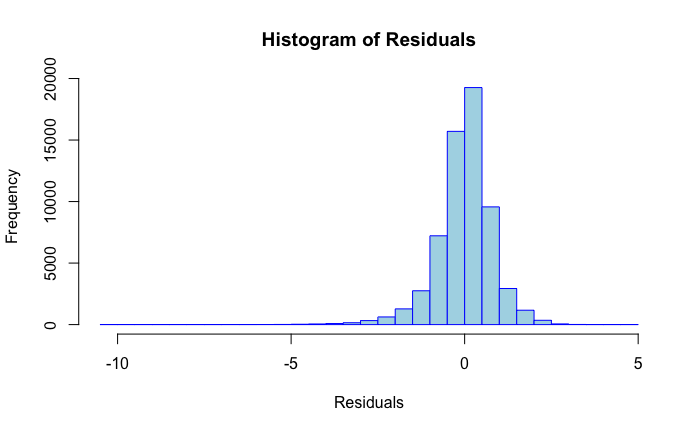
\includegraphics[width=\textwidth]{../figures/post/hist-k-foldcv.png}
    \captionof*{figure}{\textit{Residual Histogram}}
\end{minipage}
\begin{minipage}{0.49\textwidth}
    \centering
    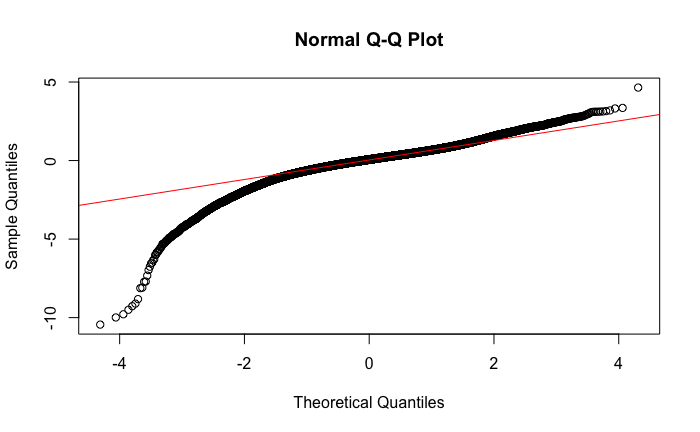
\includegraphics[width=\textwidth]{../figures/post/qq-k-foldcv.png}
    \captionof*{figure}{\textit{Residual Quantile-Quantile Plot}}
\end{minipage}
\vfill
\begin{minipage}{0.49\textwidth}
    \centering
    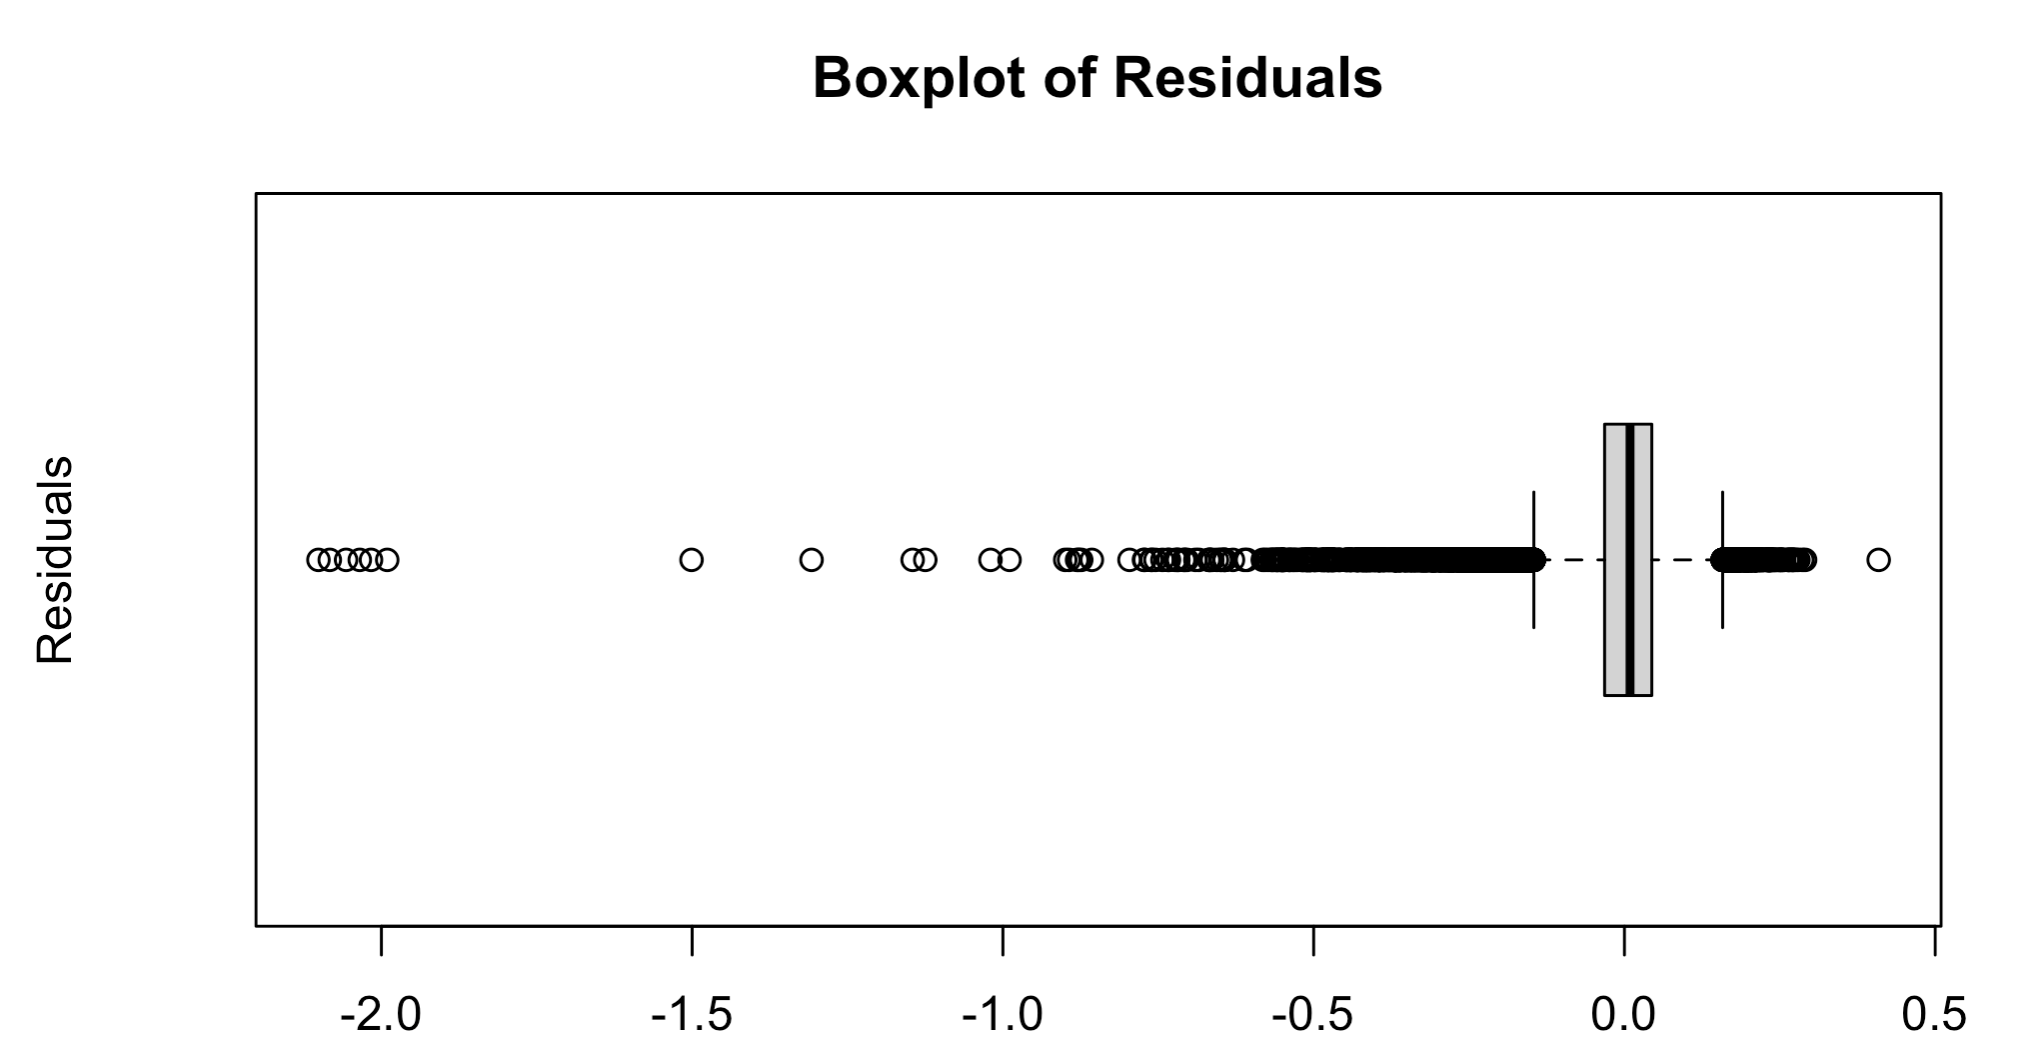
\includegraphics[width=\textwidth]{../figures/post/residual-box.png}
    \captionof*{figure}{\textit{Residual Boxplot}}
\end{minipage}
\begin{minipage}{0.49\textwidth}
    \centering
    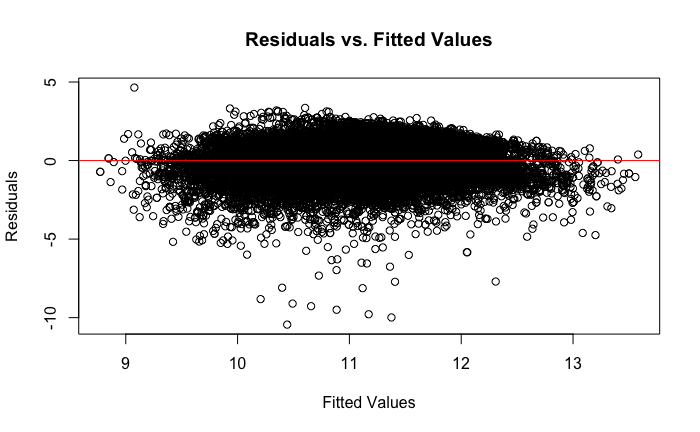
\includegraphics[width=\textwidth]{../figures/post/residualvsfitted-k-foldcv.png}
    \captionof*{figure}{\textit{Normalized Residuals vs Fitted Values}}
\end{minipage}
\vfill
\end{custommargins}
Our findings suggest that the residuals of our model are not normally distributed, therefore limiting the inferential power of our conclusions.
The quantile-quantile residual plot suggests a distribution with deviation from the reference line, which represents a normal distribution.
\\

The plot of normalized residuals vs fitted values suggests that the residuals do not have constant variance.
This suggests that our estimates of the true $\beta$ coefficients are biased. However, due to the large sample size, and the standard errors of the $\hat{\beta}$ coefficients
, we can still conclude that the positive or negative relationship between the variables and income is correct and statistically significant.
\\

The boxplot and histograms of residuals further suggests their non-normality. The presense of outliers in the lower values of \texttt{log(INCTOT)} suggests that our model may be underestimating the income of individuals with lower income.
This leads into the issues that the presense of high-income individuals has on our model and raises questions about the reliability of our seemingly good sample data.

%perhaps some more model metrics
\subsubsection*{Model Metrics}
\begin{table}[h]
    \centering
    \begin{tabular}{lr}
    \toprule
    \textbf{Statistic} & \textbf{Value} \\
    \midrule
    Residual Standard Error & 0.8194 \\
    for Degrees of Freedom= & 49256 \\
    \midrule
    Multiple R-squared & 0.2826 \\
    Adjusted R-squared & 0.2822 \\
    F-statistic & 669.1 \\
    DF for F-statistic & 29 and 49256 \\
    p-value & $< 2.2 \times 10^{-16}$ \\
    Root Mean Square Error & 0.8143115 \\
    \bottomrule
    \end{tabular}
    \caption*{Summary Statistics of the Regression Model}
\end{table}

The residual standard error was calculated to be 0.8194, which is the average difference between the observed and predicted values.
The root mean square error (RMSE) is 0.8143, which is the square root of the average of the squared differences between the observed and predicted values. In dollar amounts, the exponentiated transformation
of the residual standard error and RMSE are \$2.27 and \$2.26, respectively. This suggests that our model's predictions are only off by around \$2.26 on average,
a relatively small amount. Our model is significant, given the chosen cutoff of $\alpha=0.05$ and the model's p-value.




\clearpage
\begin{thebibliography}{9}
    \bibitem{HRfH}
    Chen, Z., Zhang, Y., Luo, H. et al. Narrowing but persisting gender pay gap among employees of the US Department of Health and Human Services during 2010–2018. \textit{Human Resources for Health}, \textbf{19}(65), 2021.
    \bibitem{BLSarticle}
    Toossi, Mitra. A Century of Change: The U.S. Labor Force, 1950-2050, May 2002, \href{www.bls.gov/opub/mlr/2002/05/art2full.pdf}{link}.
    \bibitem{issuebrief}
    Understanding the Gender Wage Gap, Women’s Bureau, Department of Labor, Mar. 2023, \href{www.dol.gov/sites/dolgov/files/WB/equalpay/WB_issuebrief-undstg-wage-gap-v1.pdf}{link}. 
    \bibitem{DallasFed}
    Liu, Sitian, and Yichen Su. “The Geography of Jobs and the Gender Wage Gap.” Federal Reserve Bank of Dallas, Working Papers, vol. 2020, no. 2028, Oct. 2020, \href{https://doi.org/10.24149/wp2028}{doi}. 
    \bibitem{public-school}
    “NCES Blog | August 26. 2022.” Nces.ed.gov, \href{nces.ed.gov/blogs/nces/2022/08/26/default}{link}.
    \bibitem{ozili}
    Ozili, Peterson K. “The Acceptable R-Square in Empirical Modelling for Social Science Research.” Papers.ssrn.com, 5 June 2022, \href{papers.ssrn.com/sol3/papers.cfm?abstract_id=4128165}{link}.

    
\end{thebibliography}

\end{document}